\documentclass[11pt,a4paper]{article}
\pdftrailerid{}
\usepackage[margin=0.82in]{geometry}
\usepackage[T1]{fontenc}
\usepackage[utf8]{inputenc}
\usepackage{lmodern,amsmath,amssymb,graphicx,booktabs,tabularx,array,float,xcolor,microtype}
% Minimal algorithm layout, using only the standard list and float packages.
\floatstyle{ruled}
\newfloat{algorithm}{htbp}{loa}
\floatname{algorithm}{Algorithm}
\newcounter{algline}
\newcounter{algdepth}
\newcommand{\algorithmicrequire}{\textbf{Input:}}
\newcommand{\algorithmicensure}{\textbf{Output:}}
\let\algrenewcommand\renewcommand
\newenvironment{algorithmic}[1][]{%
\setcounter{algline}{0}\setcounter{algdepth}{0}%
\begin{list}{}{\setlength{\leftmargin}{2.1em}\setlength{\labelwidth}{1.6em}\setlength{\labelsep}{.5em}\setlength{\itemsep}{.12em}\setlength{\parsep}{0pt}\setlength{\topsep}{.4em}}%
}{\end{list}}
\newcommand{\State}{\stepcounter{algline}\item[\scriptsize\arabic{algline}:]\hspace*{\value{algdepth}em}}
\newcommand{\Require}{\item[]\algorithmicrequire\ }
\newcommand{\Ensure}{\item[]\algorithmicensure\ }
\newcommand{\ForAll}[1]{\State\textbf{for all} #1 \textbf{do}\stepcounter{algdepth}}
\newcommand{\For}[1]{\State\textbf{for} #1 \textbf{do}\stepcounter{algdepth}}
\newcommand{\If}[1]{\State\textbf{if} #1 \textbf{then}\stepcounter{algdepth}}
\newcommand{\Else}{\addtocounter{algdepth}{-1}\State\textbf{else}\stepcounter{algdepth}}
\newcommand{\EndFor}{\addtocounter{algdepth}{-1}}
\newcommand{\EndIf}{\addtocounter{algdepth}{-1}}


\usepackage{enumitem}
\newcolumntype{Y}{>{\raggedright\arraybackslash}X}
\usepackage{hyperref}
\hypersetup{colorlinks=true,linkcolor=blue!55!black,urlcolor=blue!55!black,citecolor=blue!55!black}
\setlength{\parindent}{0pt}\setlength{\parskip}{0.55em}
\setlist[enumerate]{leftmargin=*,itemsep=3pt,topsep=4pt}
\newcommand{\du}{\Delta u}\newcommand{\dx}{\Delta x}\newcommand{\lap}{\delta_x^2}
\title{Computational Supplement:\\A Finite Bid--Ask Spread from Replenishment\\Displaced from the Quote}
\author{Christopher Angstmann \and Derick Diana \and Tim Gebbie}
\date{v1.0.0 rc1 --- Computational supplement\\3 October 2026}
\begin{document}
\maketitle
\begin{abstract}
This supplement connects the two-density spread model to its retained numerical implementation. Bid and ask liquidity evolve on a log-price lattice in operational time; explicit aggressive executions initiate delayed opposite-side replenishment whose pending volume determines supply placement. Density thresholds define the observed quotes. We distinguish external lit and latent source profiles from the aggregate dynamic densities, explain why diffusion leaves subthreshold density inside the quoted spread, and state what the market-making completion closure measures. Captioned algorithms specify the field update, execution tape, lagged correlations and declared order-flow controls. The numerical evidence comprises density and price trajectories, balanced-flow feedback comparisons, and diagnostic event-time correlations. The finite-grid spread comparisons support bounded quantitative interpretation at the retained resolution. The computations are model-conditional evidence at finite resolution; the displayed-book interpretation, dealer accounting and correlation limits are stated separately.
\end{abstract}
\clearpage
\tableofcontents
\clearpage
\section{Scientific scope}
The companion paper is Angstmann, Diana and Gebbie, \emph{A Finite Bid--Ask Spread from Replenishment Displaced from the Quote}, forthcoming preprint. This computational supplement describes the retained v0.5.6 equations, configuration and numerical outputs. The mathematical antecedents are the supplied long paper v1.1.9 and letter v1.2.0.

The scientific question is how a two-sided liquidity field responds when executions deplete one side and generate delayed supply on the other. Source placement and executable quotes are separate objects. The simulations test the finite-grid mechanism and matched feedback controls under declared synthetic inputs. F2--F4 and V1 have this finite-programme scope. F5/F6 are diagnostics whose spatial sensitivity remains unresolved. There is no market-data fit or imposed target for a square-root impact exponent.

\section{Theory-to-computation map}
\subsection{Fields, source profiles and observable liquidity}
The state is $\rho_B(x,u),\rho_A(x,u)\geq0$, the bid- and ask-side aggregate densities in one market. The coordinate $x$ is log price and $u$ is operational time. A grid cell carries volume $\rho_i\dx$; endpoint reservoirs are excluded from executable volume. In the Markov branch, the continuous notation corresponding to the retained recurrence is
\begin{equation}\label{eq:fields}
\partial_u\rho_i=D\partial_x^2\rho_i-\nu\rho_i-\kappa\rho_A\rho_B
+S_i^{\rm lit}+S_i^{\rm latent}+S_i^{\rm MM},\qquad i\in\{B,A\},
\end{equation}
with aggressive execution represented by a separate capped consumption impulse. The actual numerical ordering is given in Algorithm~\ref{alg:markov}. Diffusion aggregates repricing, cancellation removes volume, and symmetric reaction removes overlapping bid/ask density. Reaction is a field sink; it is not entered in the explicitly specified aggressor tape as an additional signed trade.

Define outward distances $d_B=q_b-x$ and $d_A=x-q_a$. The external source profiles evaluated at interior nodes are
\begin{equation}\label{eq:sources}
\begin{aligned}
S_i^{\rm lit}(x,u)&=A_{\rm lit}e^{-d_i/\ell_{\rm lit}}\mathbf1_{\{d_i\geq0\}},\\
S_i^{\rm latent}(x,u)&=A_{\rm latent}(1-e^{-d_i/\ell_{\rm latent}})\mathbf1_{\{d_i\geq0\}}.
\end{aligned}
\end{equation}
The lit term is concentrated near the outward placement edge; the latent term grows with outward distance. They are rates of supply into the same receiving field. The registered pilot uses equal amplitudes and lengths, so their sum is exactly one outside the relevant edge and zero inside it. This complementarity is a configuration choice, not an independently identified conversion process.

\begin{table}[htbp]\centering\small
\caption{Source and state meanings in the implemented two-field closure.}\label{tab:source-state}
\begin{tabularx}{\textwidth}{@{}lYY@{}}\toprule
Object & Meaning & What the implementation retains\\\midrule
$S_i^{\rm lit}$ & Near-edge external supply rate & Separate source increment before addition to $\rho_i$\\
$S_i^{\rm latent}$ & Outward external supply rate & Separate source increment before addition to $\rho_i$\\
$\rho_i$ & Aggregate dynamic side density & One evolving field per side; no lit/latent ownership labels\\
$P_i,Q_i$ & Pending opposite-side replenishment & Completion and initiation ledger; no dealer cash account\\
$C_i g_i$ & Delivered replenishment increment & Normalized outward placement; no second trade print\\
$p_b,p_a$ & Observed executable boundaries & Oriented density-threshold crossings\\
$q_b,q_a$ & Supply-placement edges & Geometry set from pending stocks\\\bottomrule
\end{tabularx}\end{table}

The source labels describe supply channels, rather than a separate stochastic order-status classification. The code does not evolve $\rho_i^{\rm lit}$ and $\rho_i^{\rm latent}$ separately, and it has no explicit latent-to-lit transition rate. Recording both source increments does not identify the subsequent density by source ancestry: the shared nonlinear reaction depends on the aggregate fields. Consequently, the figures cannot be decomposed into a measured latent part and a measured lit part of $\rho_i$. The dotted latent-book reference in the letter's schematic is also not an additive component of the numerical density or an external source. A model with separate latent and displayed stocks would require additional state variables and a specified conversion law.

\subsection{What the quoted spread measures}\label{sec:spread}
The observed bid is the rightmost downward crossing of $\rho_B=\epsilon$; the observed ask is the leftmost upward crossing of $\rho_A=\epsilon$. The crossing is linearly interpolated between nodes, with conditioning and ordering checks. Set
\begin{equation}\label{eq:quotes}
s=p_a-p_b,\qquad m=\tfrac12(p_a+p_b).
\end{equation}
The execution map consumes bid-side nodes at $x\leq p_b$ for a sell and ask-side nodes at $x\geq p_a$ for a buy, within the declared outward depth. It does not execute volume inside $(p_b,p_a)$.

A literal displayed limit-order book has no resting executable bid or ask between its best quotes at a given completed state. Equation~\eqref{eq:fields} does not impose this hard support condition on the aggregate fields. Even where all source terms vanish, diffusion imports density from neighbouring prices. Cancellation and finite-rate reaction reduce those tails without setting them identically to zero. Thus a threshold spread can coexist with positive subthreshold density between its quotes. The absence of placement between $q_b,q_a$ is a source-support statement; it is not a zero-density boundary condition, and this placement interval differs from the quoted spread.

For the stored initial F2/F3 pilot, $q_b=-6$, $q_a=6$, whereas $p_b=-4.390566$, $p_a=4.390566$ and $s=8.781131$. On the grid nodes strictly inside these observed quotes, each side's maximum density is about 0.099691, below $\epsilon=0.1$. These values are read from the saved stationary field, without evolving a new trajectory. They illustrate the threshold interpretation, rather than an empty numerical interior.

The retained fields therefore represent aggregate liquidity with an explicit executable observation rule. Their positive tails have no separately recorded order-status label. A strictly empty displayed spread would require a separate displayed/latent representation or a derived moving-support rule. The current threshold observation should be assessed on this stated basis.

\subsection{Baseline width, response and recovery}
The positive reference width is imposed through $\Sigma_0=12$, not generated from zero standoff. The quoted width also depends on $D,\nu$, source amplitudes and the observation threshold. For orientation, consider a stationary, reaction-free half-line with constant outward source $A$, fixed edge $q_b$, cancellation $\nu>0$ and distant reservoirs. Solving the two linear branches with continuity of density and derivative gives the inward tail
\begin{equation}
\rho_B(x)=\frac{A}{2\nu}e^{-(x-q_b)/\ell_\nu},\quad x\geq q_b,
\qquad \ell_\nu=\sqrt{D/\nu}.
\end{equation}
The reflected ask tail has the same form. For $0<\epsilon<A/(2\nu)$, the symmetric threshold width is
\begin{equation}\label{eq:width-reference}
s_{\rm ref}=\Sigma_0-2\ell_\nu\log\!\left(\frac{A}{2\nu\epsilon}\right),
\end{equation}
provided the selected quotes remain ordered. With $D=\nu=A=1$ and $\epsilon=0.1$, this reference gives approximately 8.7811. It explains the distinction between placement and threshold widths and their dependence on $\epsilon$. It neglects nonlinear reaction, finite reservoirs and nodal support; it is not an exact solution or a convergence test of the implemented pilot.

The simulations recover an ordered positive threshold spread and measure its displacement and relaxation after executions. F4's paired finite-grid comparisons support the accepted response at the retained resolution. ``Recovery'' does not mean that the quotes have returned exactly to their initial values by $u=8$. In the directional moving-placement pilot, the saved spread changes from 8.781131 to 8.784200, and approximately 0.000929 bid replenishment remains pending. A finite-horizon residual is not evidence of permanent impact. No empirical spread size, tick distribution or asymptotic return to equilibrium has been established.

\subsection{Market making and the meaning of a round trip}
An aggressive buy consumes ask-side volume $v_A$ and initiates bid-side replenishment; an aggressive sell consumes bid-side volume $v_B$ and initiates ask-side replenishment. The market-making sector is represented by the pending stocks and their receiving-side placement. The closure attributes the explicit child programme to this sector without simulating individual dealer balance sheets.

For the previous post-event stock $P_i$, old-cohort delivery and residual pending volume are
\begin{equation}
C_i=(1-e^{-\du/\tau_h})P_i,\qquad Q_i=P_i-C_i.
\end{equation}
The quote-setting sample uses $Q_i$, after this delivery and before the current execution:
\begin{equation}\label{eq:placement}
\begin{aligned}
Q_\Sigma&=Q_A+Q_B,& Q_\Delta&=Q_A-Q_B,\\
\Sigma&=\Sigma_0+\chi_sQ_\Sigma,&\mu&=\mu_0-\chi_mQ_\Delta,\\
q_b&=\mu-\Sigma/2,&q_a&=\mu+\Sigma/2.
\end{aligned}
\end{equation}
The delivered increment $C_i g_i$ is normalized by $\dx\sum_jg_{i,j}=1$ and placed on the receiving side, over $[q_b-w,q_b]$ or $[q_a,q_a+w]$. Newly initiated volume enters $P_B^{\rm new}=Q_B+v_A$, $P_A^{\rm new}=Q_A+v_B$ and cannot deliver in that same update.

A microscopic round trip would require two executed legs, their prices, matching or allocation of quantities, elapsed time and the resulting dealer inventory/cash account. Here the second leg is represented by completion-equivalent opposite-side supply. Its assumed delay and spatial displacement summarize the replenishment effect; they do not reconstruct an observed second execution. Delivery creates neither another aggressor sign nor another trade price. A completed volume ledger therefore establishes conservation, not earned spread or dealer profitability.

Balanced buying and selling can cancel signed pending imbalance while retaining total pending exposure. The width law responds to that gross exposure and the centre law to its sign. Even a volume-balanced programme need not immediately restore liquidity at the original quote: delivery occurs at a displaced location and subsequent transport takes time. Reaction price, quoted midpoint, placement centre and actual execution price remain distinct measurements.

\subsection{DTRW and manuscript provenance}
Diana--Gebbie identify the need for separate side densities for a nonzero spread \cite{cam}. The correlation-emergence software supplies numerical and observation antecedents \cite{ag,code}; its two coupled books are not the two sides of this single market. The fields here are independently implemented. The common Markov operator and event-ordering differences are stated below, without asserting whole-model equivalence.

\clearpage
\section{Uniform-operational simulation}
The field update, execution tape, dependence estimator and input protocol are separate algorithms. Their inputs and outputs specify what is generated, what is measured and what is merely supplied as an experimental control.

\subsection{Executable field update}
Both sides read the same frozen incoming field. With $\bar i$ denoting the opposite side and $a=D\du/\dx^2$, the pre-execution recurrence on interior nodes is
\begin{equation}\label{eq:recurrence}
\begin{split}
\widetilde\rho_{i,j}={}&(1-2a-\nu\du-\kappa\du\rho_{\bar i,j})\rho_{i,j}
+a(\rho_{i,j-1}+\rho_{i,j+1})\\
&+\du(S_{i,j}^{\rm lit}+S_{i,j}^{\rm latent})+C_i g_{i,j}.
\end{split}
\end{equation}
The delivered volume $C_i$ is already integrated over the update; multiplying its increment by $\du$ again would change the model. A sufficient nonnegativity condition is $2a+\nu\du+\kappa\du\rho_{\bar i,j}\leq1$ at every interior node. Fixed endpoint reservoirs enter transport but are excluded from execution.

\begin{algorithm}[H]
\caption{Uniform-operational update with delayed opposite-side replenishment}\label{alg:markov}
\begin{algorithmic}[1]
\Require Incoming post-event field $\rho$, stocks $P_B,P_A$, grid and parameters; requests $V_B,V_A$
\Ensure Pre/post fields and quotes, actual fills, updated stocks and accounting records
\State Freeze both side densities and all incoming stocks
\State $C_i\gets(1-e^{-\du/\tau_h})P_i$; for the next-update control set $C_i\gets P_i$
\State $Q_i\gets P_i-C_i$; set $q_b,q_a$ from Eq.~\eqref{eq:placement}
\State Evaluate $S_i^{\rm lit},S_i^{\rm latent}$ using Eq.~\eqref{eq:sources}
\State Form outward nodal supports $[q_b-w,q_b]$ and $[q_a,q_a+w]$
\State Reject empty or reservoir-truncated supports; normalize $\dx\sum_jg_{i,j}=1$
\State Check the nonnegativity bound and compute Eq.~\eqref{eq:recurrence} synchronously
\State Keep reservoirs fixed; reject nonfinite or negative field values
\State Read pre-event quotes using the oriented threshold crossings in Section~\ref{sec:spread}
\State Reject selected plateaus, insufficient slopes, invalid reservoirs or unresolved quote contact
\ForAll{nonzero side requests}
\State Select interior node centres from the observed quote outward, within the execution depth
\State Visit nodes in price priority and remove at most $\widetilde\rho_{i,j}\dx$ from each
\State Record removed node volumes, actual totals $v_i$ and unfilled demand
\EndFor
\State $P_B^{\rm new}\gets Q_B+v_A$; $P_A^{\rm new}\gets Q_A+v_B$
\State Read post-event quotes; verify field budgets and the side-specific completion ledgers
\State Save source increments, quote-setting $Q$, post-event $P$ and the distinct event phases
\end{algorithmic}
\end{algorithm}
\textbf{Checks on every update.} For each side, the interior volume change is
boundary flux minus cancellation, minus symmetric reaction, plus external
supply, plus completion, minus execution. The boundary increment is
$D\du(\rho_0-\rho_1+\rho_J-\rho_{J-1})/\dx$. Reaction loss is
$\kappa\du\dx\sum_j\rho_{A,j}\rho_{B,j}$ on each side. It cancels from
imbalance and occurs twice in total density. Cumulative initiation must equal
cumulative completion plus post-event pending stock, separately by side.

\textbf{Initialization and chronology.} Relax the same positive-reaction equations
with empty pending stock and no executions to the configured residual.
Recompute geometric completion weights when $\du$ changes, retaining physical
$\tau_h$. Preserve pending tails beyond a finite plotting horizon.
An event at $u$ acts at the end of the numerical interval ending at $u$. Its pre/post fields share that timestamp but retain separate phase labels. New initiation follows consumption and cannot deliver during this same update.

\clearpage
\subsection{Actual-fill execution observations}
\begin{algorithm}[H]
\caption{Actual-fill execution prices, labels and consecutive-event increments}\label{alg:tape}
\begin{algorithmic}[1]
\Require Removed node volumes $v_{n,j}$, pre/post quotes, event time and parent identifier
\Ensure Fill tape, three price summaries, aggressor/quote/tick signs and event increments
\State Require exactly one executed aggressor side for an observed trade; zero fill creates no observation
\State $v_n\gets\sum_jv_{n,j}$; retain every nonzero fill and requested/unfilled amount
\State $z_n\gets\sum_jv_{n,j}x_j/v_n$
\State $P_n^{\rm geom}\gets e^{z_n}$; $P_n^{\rm VWAP}\gets\sum_jv_{n,j}e^{x_j}/v_n$
\State Retain pre/post bid, ask, midpoint and spread, and the placement/pending sample used
\State Record true aggressor $\varepsilon_n$ ($+1$ buy, $-1$ sell) separately from $\operatorname{sign}(z_n-m_n^{\rm pre})$
\If{this is the first trade}
\State Set the tick label to zero and first consecutive-event increments to missing
\Else
\State $r_n^m\gets m_n^{\rm post}-m_{n-1}^{\rm post}$; $r_n^T\gets z_n-z_{n-1}$
\State $\Delta s_n\gets s_n^{\rm post}-s_{n-1}^{\rm post}$; retain $|r_n^m|,|r_n^T|$
\State Update the tick label to $\operatorname{sign}(r_n^T)$ when nonzero; otherwise retain its previous nonzero value
\EndIf
\State Record the instantaneous midpoint jump $m_n^{\rm post}-m_n^{\rm pre}$ separately
\end{algorithmic}
\end{algorithm}
The primary execution log price is $z_n$. Its exponential is a geometric price average; the arithmetic price VWAP is a distinct statistic. The increment $r_n^m$ includes inter-event field evolution as well as the current execution jump.

Prices are measured from actual density consumption; there is no independent
synthetic price process. The current six same-sign children demonstrate the
measurement path only. Their sign variance is zero, so no sign ACF or LMF
claim is available from this run.

\subsection{Lagged dependence estimator}
The estimator and the registered long-run protocol below are implemented.
F5/F6 remain diagnostic because their spatial sensitivity is unresolved. For aligned finite series $X,Y$, define
\[
 \widehat C_{XY}(k)=
 \frac{\sum_{n\in I_k}(X_n-\bar X_k)(Y_{n+k}-\bar Y_k)}
 {\sqrt{\sum_{n\in I_k}(X_n-\bar X_k)^2
              \sum_{n\in I_k}(Y_{n+k}-\bar Y_k)^2}}.
\]
Each mean is taken over its own overlapping slice. Positive $k$ means $X$
leads $Y$. Save pair counts, lag units and phase alignment. Zero variance is
undefined, not zero correlation. Do not silently compress missing observations.
This reproduces the v2.0.0 executable Pearson ACF. Its supplementary text
instead prints a global-mean covariance normalization; that documentation
mismatch is not carried into this supplement.

\begin{algorithm}[H]
\caption{Overlapping-slice Pearson dependence at an executed-trade lag}\label{alg:correlation}
\begin{algorithmic}[1]
\Require Equal finite event series $X,Y$ of length at least four and integer lag $k$
\Ensure Pearson value and overlapping pair count, or an explicit inadmissibility exit
\State Reject nonfinite or unequal inputs and a lag leaving fewer than two pairs
\State Form the complete overlapping index set $I_k$; record its pair count without deleting or compressing events
\State Compute $\bar X_k$ and $\bar Y_k$ over their respective overlapping slices
\State Compute both centred sums of squares; if either is zero, reject the undefined correlation
\State Divide the centred cross-product by the product of the two slice norms
\State For an ensemble, calculate within each path first; average independent paths and retain descriptive between-path errors
\end{algorithmic}
\end{algorithm}

The long runs retain raw price paths and use $r^m,r^T,|r^m|,|r^T|$ for
price ACFs. For a positive price, $|P|=P$; an absolute log-price level depends
on the arbitrary origin. Spread-level ACFs require a checked stationary
window. Price-level ACFs, if retained, must be labelled descriptive rather
than evidence of long memory. A fixed valuation centre and fixed reservoirs
can cause mean reversion; diffusive prices are not guaranteed.

\clearpage
\subsection{Declared flow and matched market-maker controls}
No chartist or fundamentalist population is required for the current spread
question. Static sources do not already encode strategies; fixed $\mu_0$
is a valuation reference. The retained closure is unchanged.
\begin{algorithm}[H]
\caption{Declared input flow and common-tape feedback comparisons}\label{alg:controls}
\begin{algorithmic}[1]
\Require Finite event programme or seeded parent-order law, feedback settings and numerical grid
\Ensure Retained paths, actual execution tapes and pathwise dependence diagnostics
\State For the finite programme, fix six volume-0.05 children at $u=1,1.4,1.8,2.2,2.6,3$
\State Select all buys or alternating buys/sells; retain the programme through $u=8$
\State Compare delayed/moving, next-update completion, fixed, centre-only and width-only settings at their registered grids
\State Verify equal actual fills before interpreting paired finite responses
\State For long paths, draw $L\gets\min(\lfloor2(1-U)^{-1/1.5}\rfloor,512)$ and independent centred parent signs
\State Draw initial $L_0$ from $l\Pr(L=l)/E[L]$ and integer age uniformly from $0,\ldots,L_0-1$
\State Assign distinct parent identifiers, including adjacent parents with equal signs
\State Set child volume 0.002 and operational spacing 0.01; use seeds 41001--41008
\State Generate 2048 burn and 8192 retained events per path; preserve the final burn price for the first retained increment
\State Pair moving and fixed placement on the same splitting tapes; generate independent signs with seed offset 100000 and matched volume/rate
\State Compute within-path ACFs/CCFs through lag 128 using Algorithm~\ref{alg:correlation}
\State Average eight independent paths; record descriptive bands $\mathrm{mean}\pm2\,\mathrm{SE}_{\rm paths}$
\State Save pair counts, individual-path correlations, raw fills and spread half-window means
\end{algorithmic}
\end{algorithm}
The ACF observables are $\varepsilon,r^m,r^T,|r^m|,|r^T|,s$. The CCF pairs are $(\varepsilon,r^m)$, $(\varepsilon,\Delta s)$, $(r^m,r^T)$, $(r^m,\Delta s)$, $(|r^m|,s)$ and $(|r^T|,s)$. Paired controls remain paired observations, rather than additional independent replicates.

The exact stationary single-active-parent sign reference is
\[
 C_\varepsilon(k)=\frac{E[(L-k)_+]}{E[L]}.
\]
For an untruncated tail with $1<\beta<2$ this renewal benchmark has exponent
$\beta-1$, consistent with the order-splitting motivation \cite{lmf}.
The implemented capped law is not the full concurrent-parent LMF population,
and cannot establish asymptotic long memory. The configuration reserves
lags 8--64 for a possible fit; no exponent has been fitted or accepted.
Persistent signs are declared input, not memory generated by density diffusion.

\textbf{Grids and retained data.} F2/F3 use $(\dx,\du)=(0.025,0.00025)$.
F4 shows both/fixed/width-only balanced controls at $\dx=0.003125$ and
$\du=0.00000390625$.
The 12-run assessment crosses $\dx=0.00625,0.003125$ at this common step,
phases 0 (on nodes) and 0.5 (between nodes), and three feedback settings.
Thirty-nine earlier finite controls remain saved. Centre-only and interaction
comparisons remain at their previous resolution. Long-run groups and all
26 long paths are unchanged. Half-cell padding preserves reflection while
moving each reservoir by $\dx/2$; separate domain checks are retained.

\clearpage
\section{Density evolution and observed prices}
Figures F2/F3 and V1 share the finite six-buy programme. Their coarser pilot grid illustrates execution and observation; it is distinct from the refined balanced-flow comparison in F4. The executable quote, placement edge and pending stock meanings are those in Section~\ref{sec:spread} and Table~\ref{tab:source-state}.

\setcounter{figure}{1}
\begin{figure}[H]
\centering
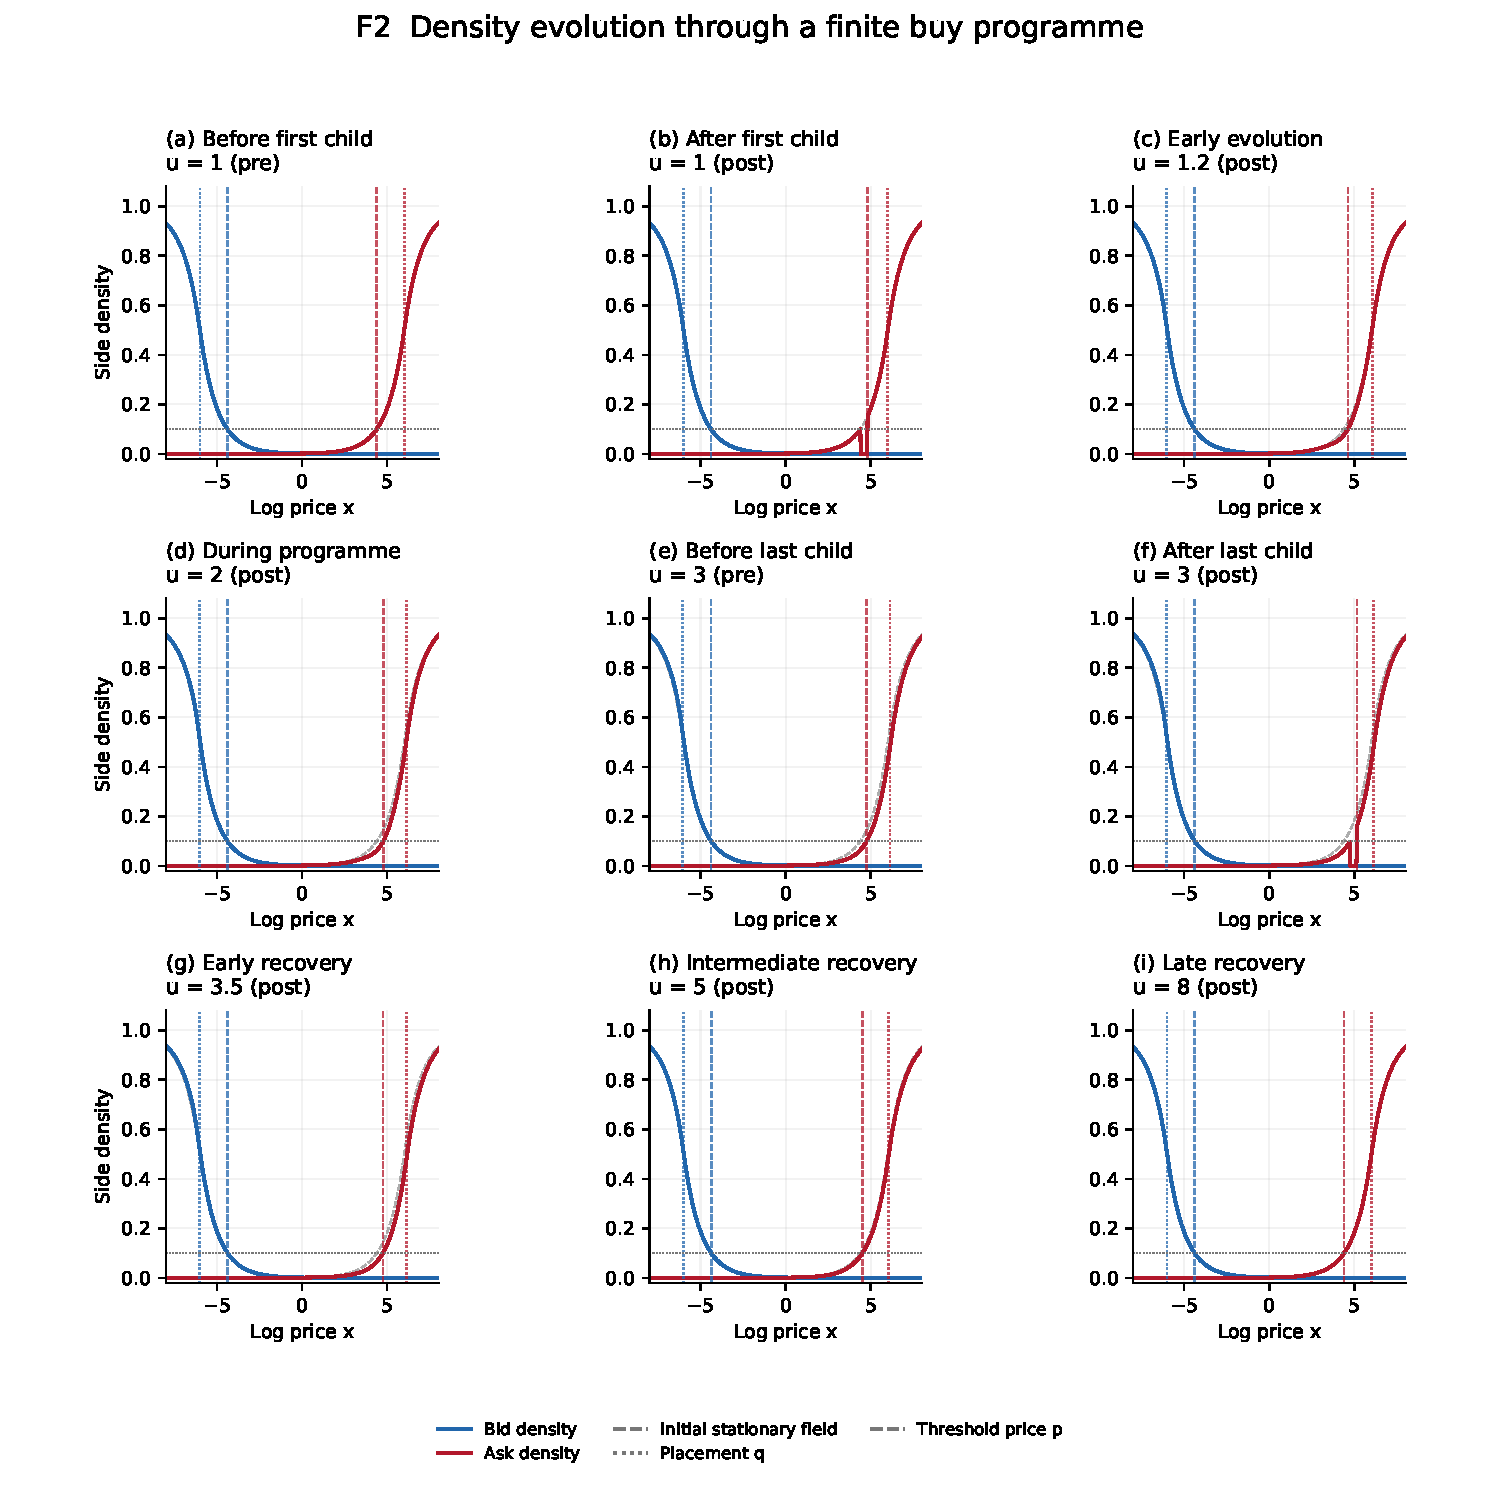
\includegraphics[width=\textwidth,height=0.55\textheight,keepaspectratio]{figures/density-v0.5.6.pdf}
\caption{\textbf{Density evolution through six buy children.}
Nine snapshots show bid density in blue, ask density in red and the relaxed
initial field in grey. Dotted lines mark placement edges and dashed lines mark
observed threshold quotes. Each child has volume 0.05, at the same times used
in F4. The grid is $\Delta x=0.025$, $\Delta u=0.00025$, the threshold is
0.1 and the computational domain is $[-12.0125,12.0125]$. The display window
is $[-8,8]$. Labelled pre/post-event pairs show immediate consumption
separately from subsequent field evolution and replenishment. These fields and threshold quotes use the observation convention in Section~\ref{sec:spread}.}
\label{fig:f2}
\end{figure}
The retained density archive stores incoming, pre- and post-consumption fields, actual removals and separate source increments. Its phase labels connect each execution to the surrounding field updates.
\clearpage
\begin{figure}[H]
\centering
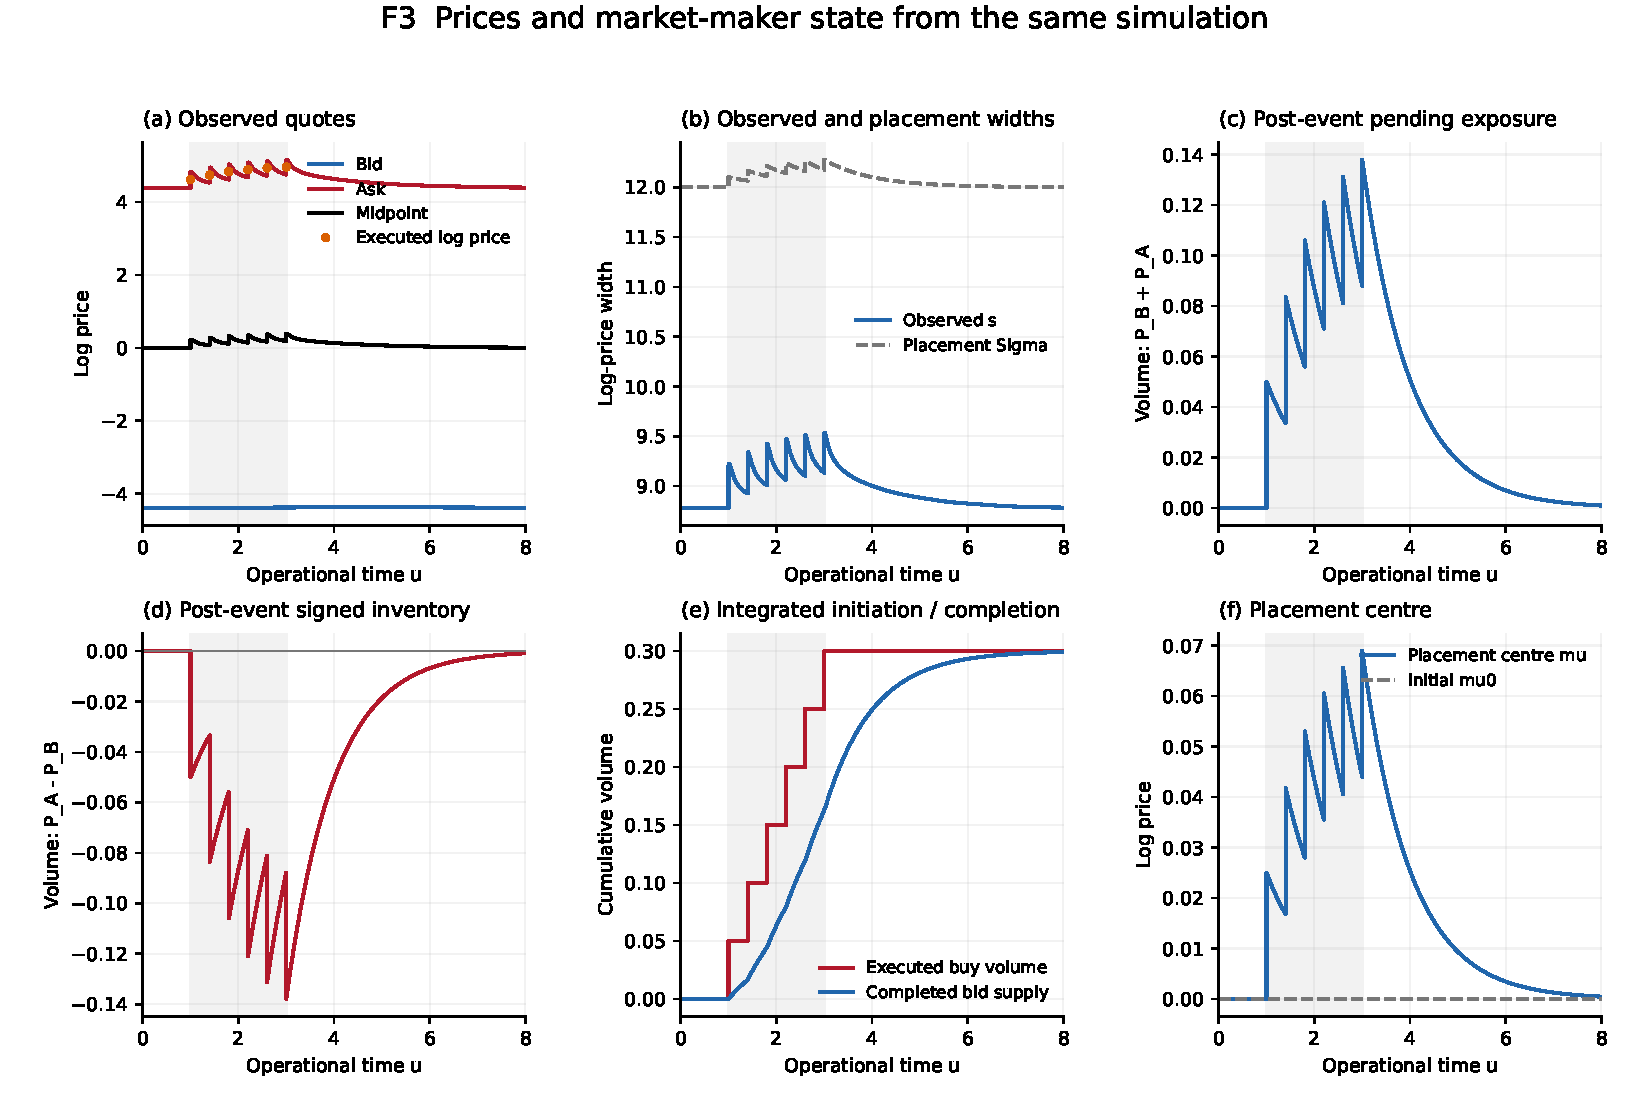
\includegraphics[width=\textwidth,height=0.55\textheight,keepaspectratio]{figures/timeseries-v0.5.6.pdf}
\caption{\textbf{Prices, placement and pending replenishment from one run.}
Panel (a) shows observed bid/ask, log midpoint and actual fill-weighted execution
log prices; (b) compares observed spread with placement width; (c,d) show
post-event total and signed pending stock; (e) records cumulative initiation
and completion; and (f) shows the placement centre. The panels share the
F2 event programme and operational-time axis. Completion is recorded in
volume units and creates no additional trade print. The execution prices use Algorithm~\ref{alg:tape}.}
\label{fig:f3}
\end{figure}
The state series records both quote-setting residual $Q$ and post-event pending stock $P$. The total-stock and imbalance panels show the distinct inputs to width and centre placement.
\clearpage
\begin{figure}[H]\centering
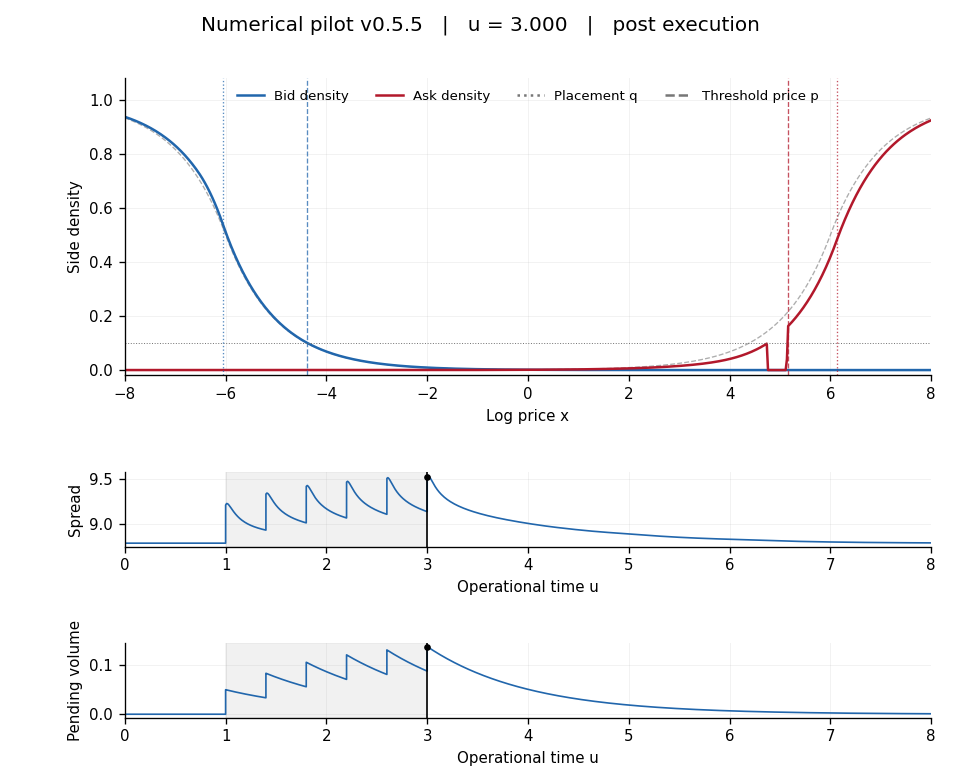
\includegraphics[width=0.8\textwidth,height=0.55\textheight,keepaspectratio]{figures/video-poster-v0.5.6.png}
\renewcommand{\thefigure}{V1}
\renewcommand{\theHfigure}{v1}
\caption{\textbf{Density trajectory through six aggressive executions.} Poster from the unchanged 24-second movie. The upper panel shows bid/ask fields, initial reference and placement/threshold edges; lower panels track quoted spread and total pending replenishment. Fixed axes and operational-time/phase labels identify held states. Consecutive pre/post frames separate consumption from later field evolution, without interpolation across impulses. Playback time is a presentation coordinate. The frame index records the actual operational time and phase.}\label{fig:v1}
\end{figure}
\addtocounter{figure}{-1}
\href{https://github.com/timgebbie/two-field-spread-reproducibility/blob/main/figures/density-v0.5.6.mp4}{Video V1: density-v0.5.6.mp4}. The poster and movie use the same saved F2/F3 trajectory. The film illustrates the mechanism; the paired numerical assessments provide its quantitative resolution evidence.
\newpage
\section{Balanced-flow response and numerical resolution}
The verified numerical baseline passes 29 focused tests. Twelve balanced controls retain the six alternating
0.05 children, horizon 8 and completion law. Each grid initializes independently
to rate-residual $10^{-8}$. Settings are both feedbacks, fixed placement and
width only ($\chi_m=0$). At $\dx=0.00625$, compare the new
$\du=0.00000390625$ against retained $\du=0.000015625$ (time).
Compare $\dx=0.00625,0.003125$ at the new common step (space).

For $y=m,s$, retain $R_k(u)=y_k(u)-y_k(0)$ and the matched effect
$E_k(u)=R_k(u)-R_{\rm fixed}(u)$. Report their grid differences without
allocating additive causal shares. Matched fills give equal pending schedules;
the evolving densities can differ.

\begin{table}[H]\centering\small
\caption{Paired time and spatial spread comparisons for the retained balanced programme. Phase 0 places the initial supply edges on nodes and phase 0.5 between nodes. Maxima use common 0.02 output times, with post-event states at the children. The unchanged 0.01 tolerance applies to absolute spread; response differences have no separate acceptance tolerance. Values below are rounded to six decimals.}\label{tab:refinement}
\begin{tabular}{lllrr}
\toprule
Check & Phase & Feedback & Max. spread diff. & Max. response diff.\\
\midrule
Time & 0.0 & Both & 0.000015 & 0.000015 \\
Space & 0.0 & Both & 0.005198 & 0.004393 \\
Time & 0.0 & Fixed & 0.000015 & 0.000015 \\
Space & 0.0 & Fixed & 0.005198 & 0.002078 \\
Time & 0.0 & Width only & 0.000015 & 0.000015 \\
Space & 0.0 & Width only & 0.005198 & 0.004392 \\
Time & 0.5 & Both & 0.000015 & 0.000015 \\
Space & 0.5 & Both & 0.002383 & 0.002378 \\
Time & 0.5 & Fixed & 0.000015 & 0.000015 \\
Space & 0.5 & Fixed & 0.002073 & 0.002078 \\
Time & 0.5 & Width only & 0.000015 & 0.000015 \\
Space & 0.5 & Width only & 0.002735 & 0.002730 \\
\bottomrule
\end{tabular}
\end{table}
All twelve absolute-spread comparisons meet the stated 0.01 tolerance.
Maximum spread-response differences are 0.00001486 (time) and
0.00439334 (space).
These finite comparisons do not establish a convergence order or the continuum
limit. No new response tolerance is chosen. Both phases are retained. Maxima
use common 0.02 output times and post-event states at children, not every update.

\clearpage
\begin{figure}[H]
\centering
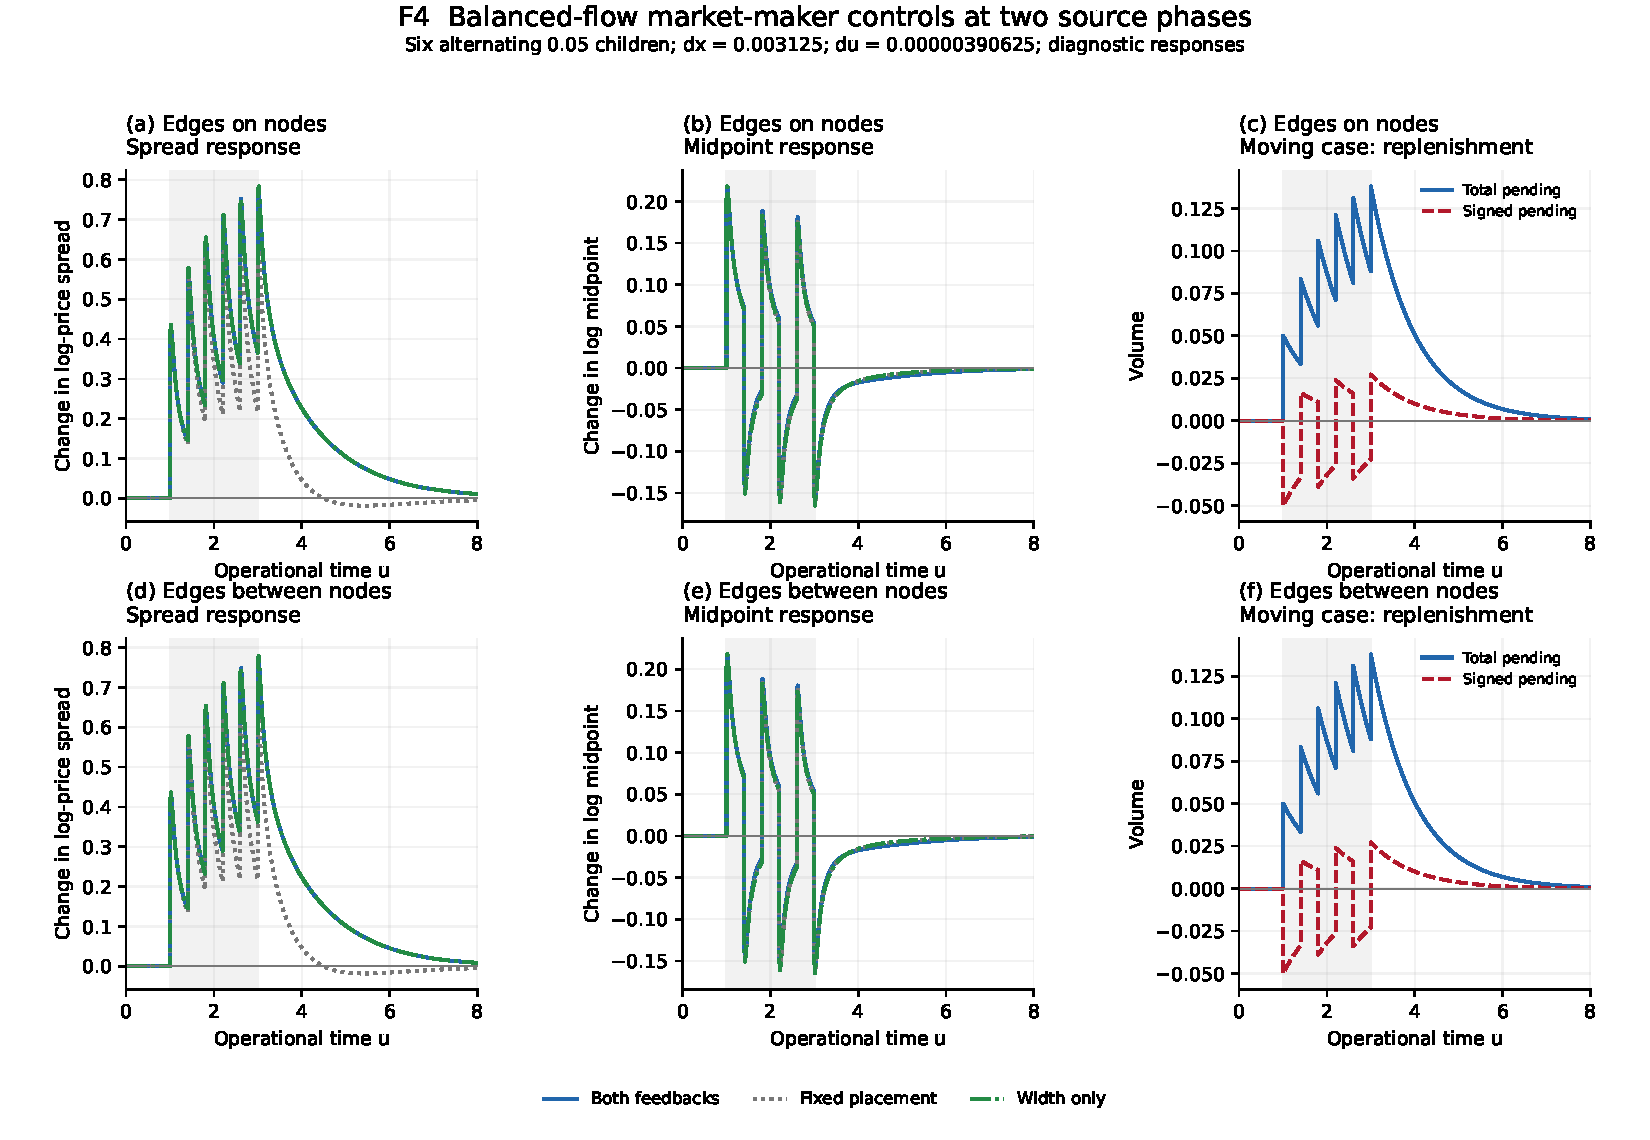
\includegraphics[width=\textwidth,height=0.55\textheight,keepaspectratio]{figures/controls-v0.5.6.pdf}
\caption{\textbf{Spread response under balanced buying and selling.}
Panels (a,d) show the change in quoted spread, (b,e) the change in log
midpoint, and (c,f) total and signed pending replenishment in the moving case.
The upper row places the initial supply edges on lattice nodes; the lower row
places them between nodes. Blue curves use both width and centre feedback,
grey dotted curves use fixed placement, and green dash-dotted curves use width
feedback alone. Each programme contains six alternating buy/sell children of
volume 0.05 at $u=1,1.4,1.8,2.2,2.6,3$, followed to $u=8$.
Responses subtract each case's stationary initial value. The grid is
$\Delta x=0.003125$, $\Delta u=0.00000390625$; corresponding columns have
common axes, and pre/post-event values retain the execution jumps. The comparisons resolve a finite-grid response; width and centre effects are not allocated additive causal shares.}
\label{fig:f4}
\end{figure}
Each programme fills 0.3 with unfilled volume below $10^{-12}$. Maximum
field/ledger errors are $3.6\times10^{-15}$/$6.2\times10^{-15}$.
Accounting and admissibility are checked every update. The assessment also
checks matched pending stocks and placement formulas. Fixed-control effects
are retained; centre-only and nonlinear interaction stay at their prior resolution.

The six successive spatial response differences decrease in both source phases for both/fixed/width-only feedback. Together with the time comparisons, they support qualitative and bounded quantitative interpretation of this finite-grid response. Centre-only and interaction results retain their earlier resolution. The comparison estimates are evaluated on the common saved-time grid, and establish neither a convergence order nor a continuum limit.

\clearpage
\section{Event-time dependence diagnostics}
The long tapes use declared parent-sign persistence and actual density consumption. They investigate how supplied sign memory appears in midpoint, execution-price and spread statistics, with fixed-placement and independent-sign controls. The exact renewal sign reference validates the input construction; it does not establish that price memory emerges endogenously or that the model reproduces a universal market law.

\begin{figure}[H]
\centering
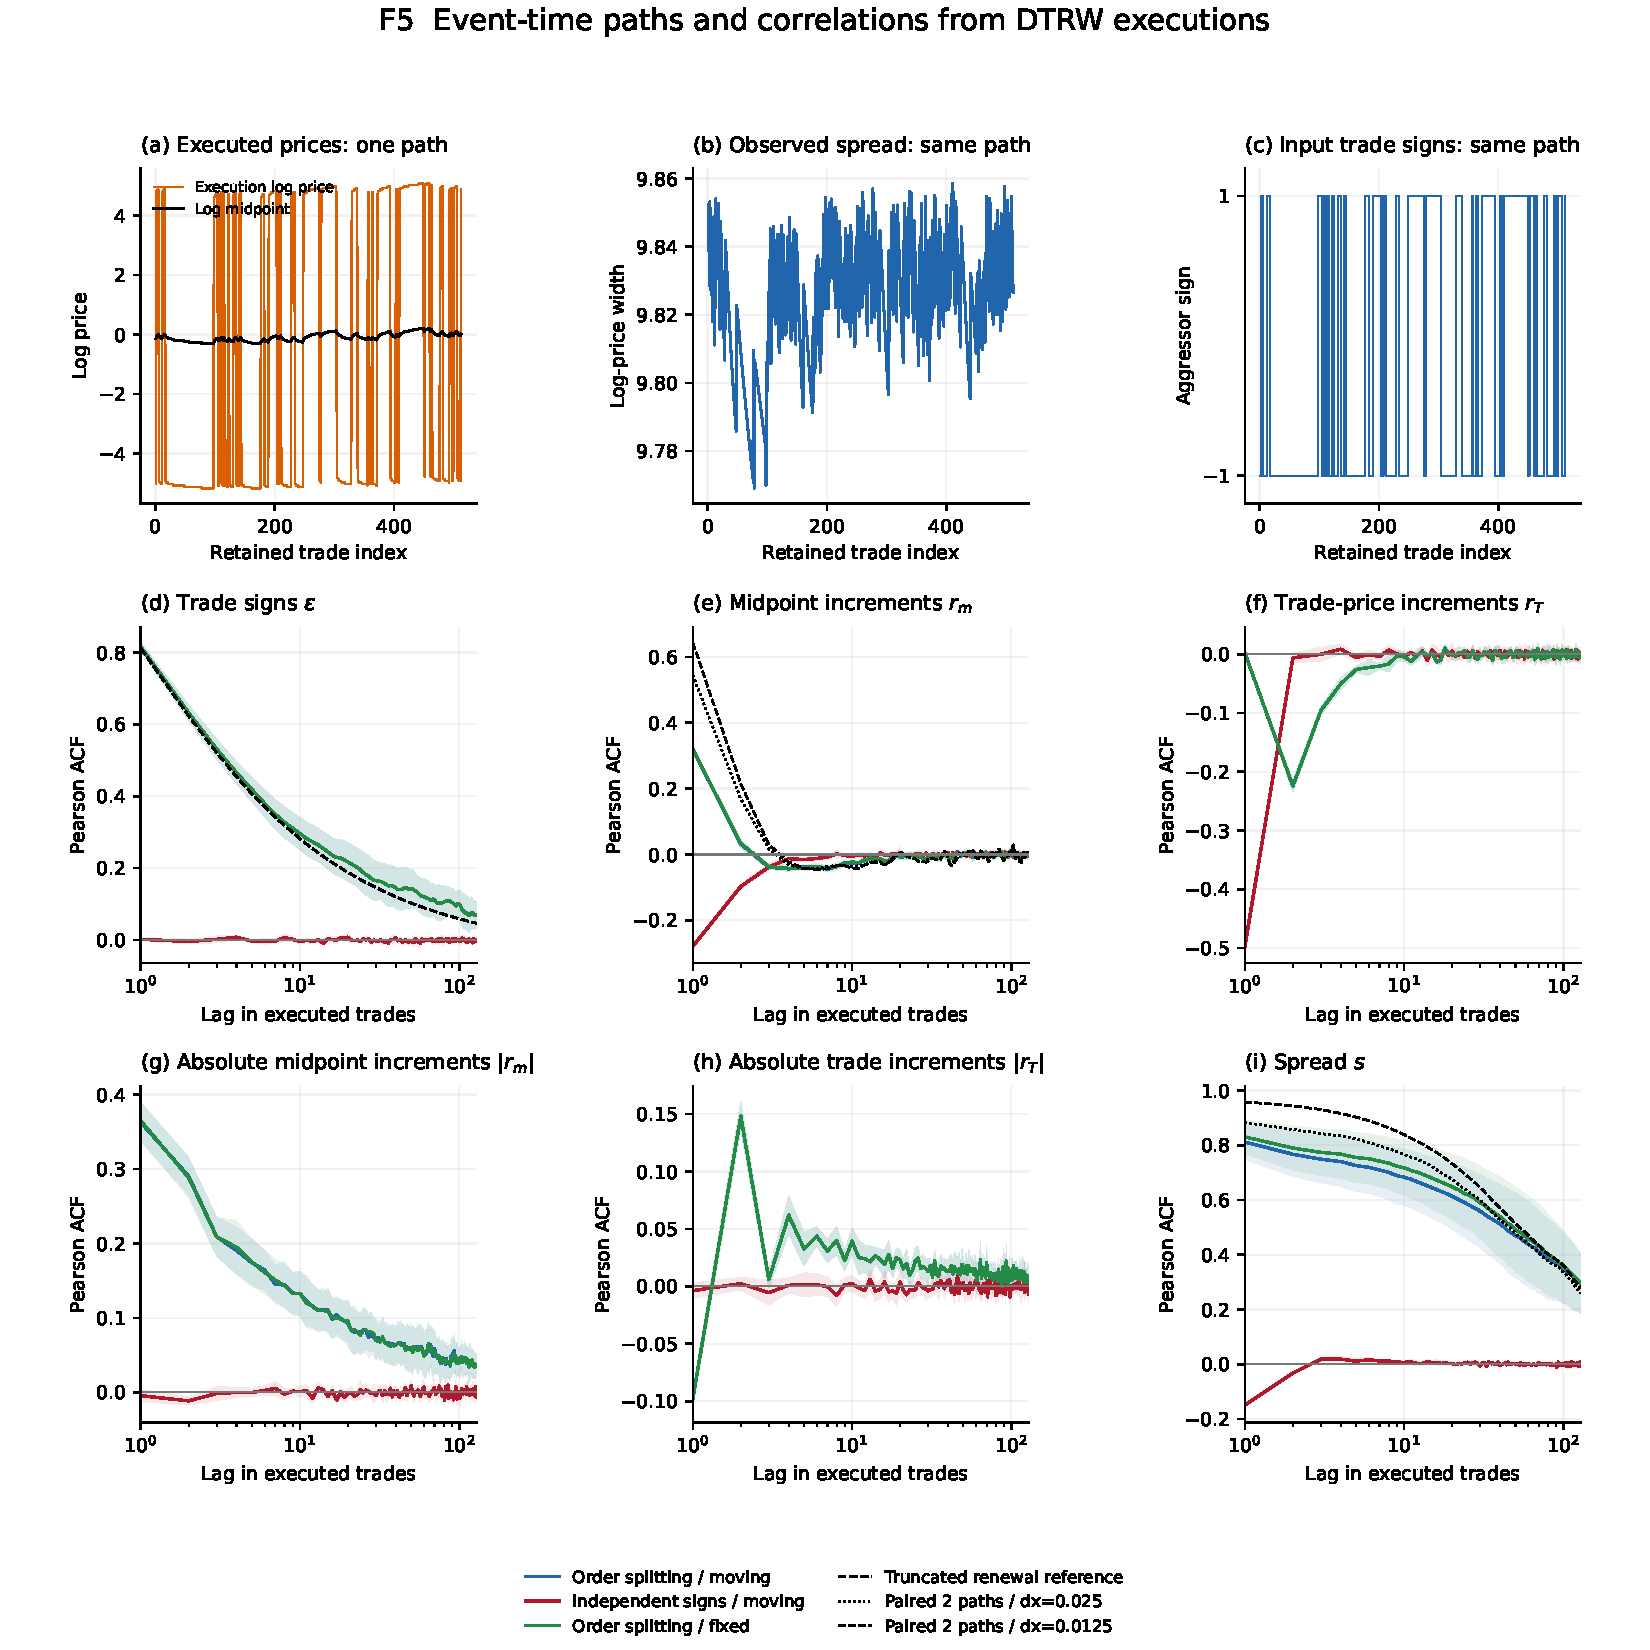
\includegraphics[width=\textwidth,height=0.55\textheight,keepaspectratio]{figures/autocorrelations-v0.5.6.pdf}
\caption{\textbf{Declared sign memory and the resulting execution statistics.}
The upper row shows execution log price and log midpoint, observed spread,
and aggressor signs for the first 512 retained events of seed 41001.
The remaining panels show ACFs of signs, midpoint increments, execution-price
increments, their absolute increments, and spread. Blue curves use order
splitting with moving placement, red curves independent signs with moving
placement, and green curves the same splitting tapes with fixed placement.
Each coloured mean uses eight independent paths with 2048 burn events and
8192 retained events, child volume 0.002 and spacing 0.01 in operational time.
Shading is the mean plus or minus two between-path standard errors. The coloured paths use $\Delta x=0.05$, $\Delta u=0.001$.
The dashed sign reference is the exact finite-cap stationary renewal
correlation $C_\varepsilon(k)=\mathbb{E}[(L-k)_+]/\mathbb{E}[L]$.
Black midpoint/spread curves compare two matched full tapes at
$\Delta x=0.025$ and $0.0125$, with common $\Delta u=0.0000625$;
they have no ensemble band. Lags count executed trades. The ACF estimator
centres each overlapping slice separately. Bands are descriptive between-path mean errors. Midpoint/spread correlations remain spatially sensitive; no limiting law or whitening is established.}
\label{fig:f5}
\end{figure}
\clearpage
\begin{figure}[H]
\centering
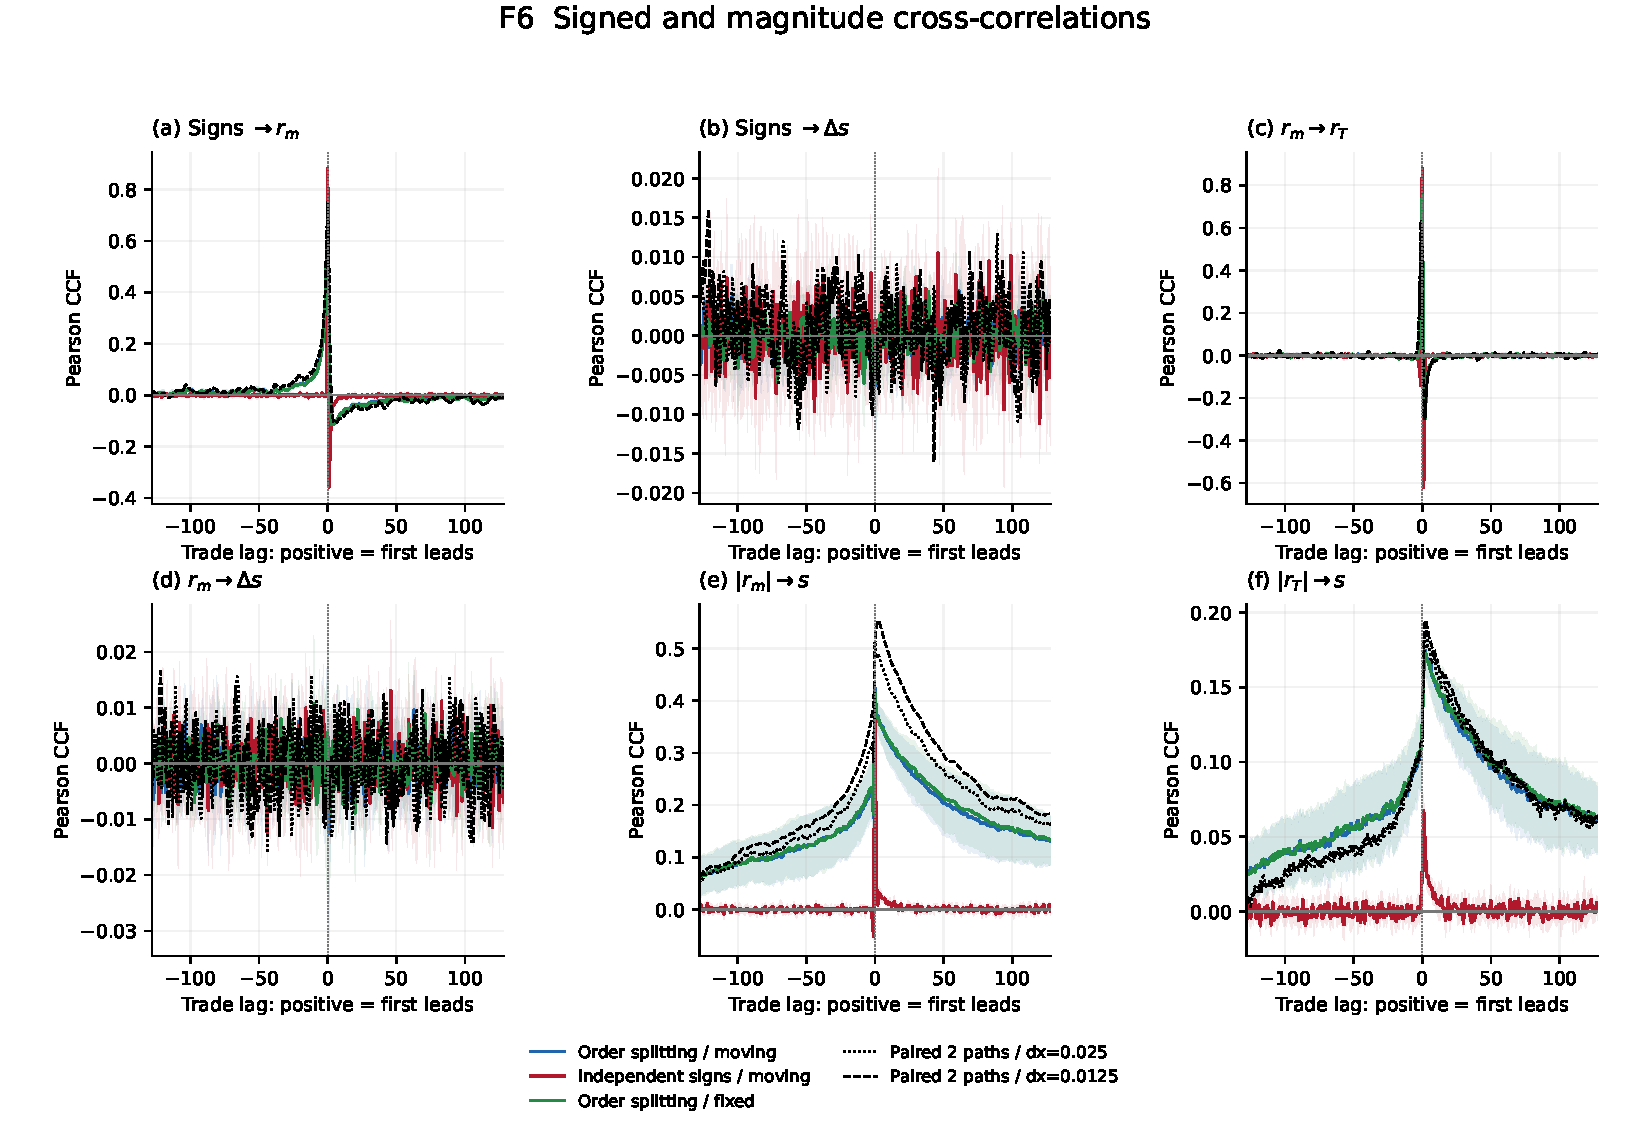
\includegraphics[width=\textwidth,height=0.55\textheight,keepaspectratio]{figures/cross-correlations-v0.5.6.pdf}
\caption{\textbf{Lagged dependence among executed flow, price increments and spread.}
Panels (a--f) show $(\epsilon,r_m)$, $(\epsilon,\Delta s)$,
$(r_m,r_T)$, $(r_m,\Delta s)$, $(|r_m|,s)$ and $(|r_T|,s)$, respectively.
Here $r_m$ and $r_T$ are consecutive-execution increments in log midpoint and
execution log price. Colours, path ensembles, shading and black paired-grid
curves follow F5. Positive lag means the first observable leads the second.
The two rows share the signed trade-lag convention and zero-lag reference. Signed cancellation and magnitude dependence answer different questions; spatial sensitivity remains unresolved and correlation does not identify causality.}
\label{fig:f6}
\end{figure}
The retained full-tape spatial comparisons change midpoint and spread ACFs by up to 0.10340 and 0.12893. Fine-grid lag-one midpoint ACF is 0.636--0.651. These measured differences leave the long-path statistics diagnostic; they do not inherit the finite-programme spread acceptance.

\section{Numerical evidence and reproducibility}
The verified runtime is Python 3.12.14, NumPy 2.3.5 and Matplotlib 3.10.8 on Linux, with FFmpeg/libx264 for V1 and pdfLaTeX for this document. Verification covers the 29 focused tests, saved-data diagnoses, five PNG/PDF pairs and V1. Windows execution remains unverified. This revision uses the retained fields and paths.

The active configuration is \texttt{config/}\allowbreak\texttt{experiments-v0.5.6.json}. Numerical code, filenames and the manifest retain that identity. Algorithm~\ref{alg:markov} maps to \texttt{functions/core.py}; Algorithm~\ref{alg:tape} to \texttt{functions/}\allowbreak\texttt{observables.py}; dependence maps to \texttt{functions/observables.py} and input controls to \texttt{functions/experiments.py}. \texttt{scripts/run\_all.py --diagnose-only} verifies saved input/data hashes and reproduces diagnoses; \texttt{--render-only} redraws figures from saved states in a separate validation copy. The default runner evolves the full numerical programme; the two saved-data routes separate evidence verification from trajectory generation.

\subsection{Parameters and evidence files}
All experiment inputs are dimensionless and illustrative. Volume is measured by the grid quadrature $\rho_i\dx$, and $x$ is a log-price coordinate. The common physical coefficients remain fixed across the registered grid comparisons.
\begin{table}[H]\centering\small
\caption{Common model parameters and observation settings. Pilot and refined-control grids are identified in the figure captions; long-path coarse and paired grids are stated in F5.}\label{tab:parameters}
\begin{tabularx}{\textwidth}{@{}l l Y@{}}\toprule
Parameter & Value & Role\\\midrule
$D,\nu,\kappa$ & $1,1,0.5$ & Diffusion, cancellation and symmetric reaction\\
$A_{\rm lit},A_{\rm latent}$ & $1,1$ & External source amplitudes\\
$\ell_{\rm lit},\ell_{\rm latent}$ & $1,1$ & External source lengths\\
$\Sigma_0,\mu_0$ & $12,0$ & Empty-pending placement width and centre\\
$\chi_s,\chi_m$ & $2,0.5$ & Total-stock width and signed-stock centre feedback\\
$\tau_h,w$ & $1,0.5$ & Completion time and outward placement support width\\
$\epsilon$ & $0.1$ & Observed-quote density threshold\\
Execution depth & $2$ & Outward extent eligible for aggressive consumption\\
Minimum selected slope & $10^{-6}$ & Conditioning check for threshold interpolation\\
Stationary rate residual & $10^{-8}$ & Independent grid initialization stopping criterion\\\bottomrule
\end{tabularx}\end{table}

\begin{table}[H]\centering\small
\caption{Figure-to-data map for the retained reproducibility evidence. All files below are in \texttt{outputs/} and carry the suffix \texttt{-v0.5.6}.}\label{tab:evidence}
\begin{tabularx}{\textwidth}{@{}lYY@{}}\toprule
Output & Stored evidence & Main archive or series stem\\\midrule
F2, V1 & Side-density states and frame phases & \texttt{density.npz}, \texttt{density-index.csv}, \texttt{video-frames.csv}\\
F3 & Prices, fills and completion stocks & \texttt{moving.csv}, \texttt{moving-trades.csv}\\
F4 & Common-input controls and paired grid errors & \texttt{market-maker.npz}, \texttt{control-comparisons.json}\\
F5, F6 & Event paths, per-path and ensemble correlations & \texttt{statistics-paths.npz}, \texttt{correlations.npz/csv}\\\bottomrule
\end{tabularx}\end{table}
For example, the stem \texttt{density.npz} denotes \texttt{density-v0.5.6.npz}. The source/data manifest verifies the numerical inputs and saved outputs before diagnosis or rendering. Exact field and completion budgets are independent of the finite-grid comparison tolerance.

\subsection{Component compatibility}
For the common reaction-free interior operator, the prototype has
\[
 \rho^{n+1}=e^{-\nu\du}\rho^n+\tfrac r2\lap\rho^n+\du S^n,
 \qquad r=2D\du/\dx^2,
\]
where $\lap\rho_j=\rho_{j-1}-2\rho_j+\rho_{j+1}$. Here cancellation is
$(1-\nu\du)\rho^n$. Their difference is
$(e^{-\nu\du}-1+\nu\du)\rho^n$, of one-step order $\du^2$.
Matched transport agrees to roundoff at $\nu=\kappa=0$; complete trajectories
are not asserted identical. The prototype consumes before its field update;
the present paper convention consumes after it. Phase labels preserve this
distinction. See \texttt{compatibility-v0.4.1.json} for the executed comparison.

\clearpage
\section{Interpretive limits}
The accepted result is a threshold-defined finite spread response under the stated source geometry and matched feedback controls. Baseline standoff, threshold and reservoirs remain structural inputs. Hard nodal supports and node-centre execution have retained resolution effects. The directional pilot is not the refined balanced comparison, and neither figure validates an empirical displayed-book gap. Separate latent/lit states, individual dealer round trips and cash accounting are outside the current closure. Centre-only and interaction precision remains at the earlier grid. F5/F6 do not establish asymptotic long memory, a square-root law or universal volatility clustering.

The supplied long paper and current letter retain their identities. The reaction price is a zero of the imbalance, whereas the quoted midpoint is formed from threshold quotes; post-execution imbalance zeros need not be unique. Distributed outward placement is not replaced by a point-at-edge approximation. Density response, first passage and the assumed completion lag are distinct kernels. These qualifications preserve the scientific interpretation without changing the recurrence or either manuscript.

\subsection{Possible memory and observation extensions}
Keep four mechanisms distinct: event-time order splitting ($\beta$),
operational transport memory ($\alpha_u$), round-trip completion ($h,\tau_h$)
and calendar observation/subordination ($\alpha_t$). Use separate recorded random streams for stochastic components. The event/operational/calendar
distinction also follows the companion account \cite{clocks}; its abstract
provides context here, not verification of a fractional two-side solver.

The prior raw Sibuya kernel is
\[
 K_1=\alpha_u,\qquad K_2=\tfrac12\alpha_u(\alpha_u-1),\qquad
 K_k=K_{k-1}\left(1-\frac{2-\alpha_u}{k}\right),\ k\geq3.
\]
The prototype applies survival $e^{-\nu(k-1)\du}$ to lagged transport
and $e^{-\nu\du}$ to the current survivor, once each. Cancellation is not
already folded into the raw kernel. $\alpha_u=1$ leaves only $K_1=1$.
Its scaling is $D_{\alpha_u}=r\dx^2/(2\du^{\alpha_u})$; changing
$\alpha_u$ while silently retaining an incompatible $r,\du,D$ is invalid.

The current state has no transport-history buffer. A future fractional
two-side model must derive the survival and history treatment of nonlinear
reaction, cancellation, births and consumed volume. It must not resurrect
removed liquidity through old history. This requires a stated formulation
and tests against the prior primitive and its Markov limit; inserting the
kernel into the existing Laplacian alone is insufficient.

The paper's stationary placement construction requires a finite mean
completion lag. A heavy-tailed transport waiting time is not permission to
replace the completion density with an infinite-mean law. That would change
the equilibrium assumptions and can make pending exposure diverge under
sustained input.

The correlation-emergence observation layer acts on completed operational
paths. A future projection must select the previous completed state under
the declared clock, retain index maps and reject out-of-support queries.
Do not interpolate across an execution. Use a coherent book observation for
bid, ask and midpoint before testing separate reporting delays. A held last
trade price creates neither another trade nor another sign. Empty calendar
bins have zero signed flow, not a repeated aggressor; distinguish them from
missing pre-first-trade observations. Compare shocked/control paths using
the same realized clock. These are specifications for a future observation layer.

\clearpage
\begin{thebibliography}{9}\small
\bibitem{cam} D. Diana and T. Gebbie, \emph{Non-uniformly sampled simulated
price impact of an order-book}, Journal of Computational and Applied
Mathematics \textbf{456} (2025), 116202.
\href{https://doi.org/10.1016/j.cam.2024.116202}{doi:10.1016/j.cam.2024.116202}.
\bibitem{ag} C. N. Angstmann and T. Gebbie, \emph{Correlation emergence and
the Epps effect in two coupled limit order books},
\href{https://arxiv.org/abs/2606.14182}{arXiv:2606.14182}, version 3.
\bibitem{code} T. Gebbie, \emph{correlation-emergence-reproducibility},
\href{https://github.com/timgebbie/correlation-emergence-reproducibility/releases/tag/v2.0.0}{v2.0.0}
and \href{https://github.com/timgebbie/correlation-emergence-reproducibility/releases/tag/v2.2.0}{v2.2.0}.
Exact commits and inspected component hashes are in \texttt{SOURCES.md}.
\bibitem{lmf} F. Lillo, S. Mike and J. D. Farmer, \emph{A theory for
long-memory in supply and demand}, Physical Review E \textbf{71} (2005),
066122. \href{https://arxiv.org/abs/cond-mat/0412708}{arXiv:cond-mat/0412708}.
\bibitem{impact} J. Donier, J. Bonart, I. Mastromatteo and J.-P. Bouchaud,
\emph{A fully consistent, minimal model for non-linear market impact},
\href{https://arxiv.org/abs/1412.0141}{arXiv:1412.0141}.
\bibitem{clocks} C. Angstmann and T. Gebbie, \emph{Event-Time Order-Flow
Memory, Operational-Time Impact, and Subordinated Market Observables},
\href{https://arxiv.org/abs/2609.13715}{arXiv:2609.13715} (2026).
\end{thebibliography}
\end{document}
